\chapter{Background and Literature Review}
\label{chap:background}

Testing for equal MI in two populations requires an estimate from each
sample and its sampling variance. This chapter develops the MI estimator,
derives its variance, and reviews tests for equal population MI.

\section{Information-theoretic foundations}

\subsection{Entropy and information content}

Entropy measures uncertainty about a variable's value, and MI measures how
much that uncertainty is reduced, on average, by observing another variable
\citep{shannon1948}.

For a discrete random variable \(X\) with probability mass function
\(p_X(x)\), the information content of outcome \(x\) is
\(-\log p_X(x)\).
Rare outcomes have larger information content because they are less expected.
The Shannon entropy is the expected information content, measured here in
nats using natural logarithms:
\begin{equation}
  H(X)=-\sum_x p_X(x)\log p_X(x).
  \label{eq:entropy}
\end{equation}

For a pair \((X,Y)\), the joint entropy \(H(X,Y)\) is defined from the joint
probabilities in the same way. The conditional entropy
\(
H(X\mid Y)=H(X,Y)-H(Y)
\)
measures the uncertainty remaining in \(X\) after observing \(Y\).

\subsection{Pointwise and average mutual information}

Let \(P=(p_{ij})\) be the joint distribution of categorical variables
\(X\in\{1,\ldots,r\}\) and \(Y\in\{1,\ldots,c\}\).
The numbers of categories, \(r\) and \(c\), are their alphabet sizes. Write
\begin{equation}
  p_{i+}=\sum_{j=1}^{c}p_{ij},
  \qquad
  p_{+j}=\sum_{i=1}^{r}p_{ij}
\end{equation}
for the marginal probabilities, or row and column margins. The pointwise
mutual information (also called local MI) associated with cell \((i,j)\) is
\begin{equation}
  \pmi_P(i,j)
  =\log\left(\frac{p_{ij}}{p_{i+}p_{+j}}\right).
  \label{eq:background-pmi}
\end{equation}
The denominator is the cell probability under independence with the same
margins. Positive pointwise MI means that the cell occurs more often than
independence predicts, whereas negative pointwise MI means that it occurs
less often.

Mutual information is the probability-weighted average of these pointwise
values \citep{shannon1948,bossomaier2016}:
\begin{equation}
  I(P)
  =\sum_{i=1}^{r}\sum_{j=1}^{c}p_{ij}\pmi_P(i,j).
  \label{eq:background-mi}
\end{equation}
Here the summations are nested: for each row \(i\), the inner sum runs over
all columns \(j\). Equivalently, the expression sums once over every cell in
the table and may be written with the shorthand \(\sum_{i,j}\).

Because \(P\) is the joint distribution of \((X,Y)\), we also write
\(I(P)\) as \(I(X;Y)\). Its entropy form is
\begin{equation}
  I(X;Y)=H(X)+H(Y)-H(X,Y).
  \label{eq:mi-entropy-form}
\end{equation}
MI is therefore the average reduction in uncertainty about \(X\) obtained
by observing \(Y\), or equivalently about \(Y\) obtained by observing \(X\).
It is nonnegative and equals zero exactly when
\(p_{ij}=p_{i+}p_{+j}\) for every cell, including zero-probability cells
\citep{bossomaier2016}.

Although MI measures the overall departure from independence, it does not
specify the shape of association. Two populations can have the same MI while assigning
probability to different cells, having different margins, or exhibiting
different association patterns. Equality of MI is therefore weaker than equality of distributions, so
the null hypothesis requires equal MI without requiring identical cell
probabilities in the two population tables.

The logarithm base determines the reporting unit, and this thesis uses
natural logarithms to express MI in nats. Dividing by \(\log 2\)
converts MI to bits by rescaling MI and its standard error together,
while leaving the degrees of freedom unchanged. The test result is
therefore identical in either unit.

\section{Estimating discrete mutual information}
\label{sec:background-mi-bias}

Suppose a sample of size \(n\) produces counts \(N_{ij}\). The empirical cell
probabilities are
\begin{equation}
  \widehat p_{ij}=\frac{N_{ij}}{n}.
\end{equation}
The plug-in estimator inserts these observed relative frequencies into
Equation~\eqref{eq:background-mi}:
\begin{equation}
  \Ihat(P)
  =\sum_{i,j:\widehat p_{ij}>0}
  \widehat p_{ij}
  \log\left(
  \frac{\widehat p_{ij}}
       {\widehat p_{i+}\widehat p_{+j}}
  \right).
  \label{eq:plugin-mi-background}
\end{equation}
The zero-cell convention follows from
\(\lim_{x\downarrow0}x\log x=0\), so empty cells contribute no term to
the sum. When a positive-probability cell is unobserved, the empirical
table assigns it zero probability, contributing to sparse-sample estimation
error.

When the counts follow a multinomial distribution, they vary between samples
but must sum to \(n\), so an extra observation in one cell leaves fewer
observations for the others. For a fixed set of categories, the plug-in
estimate approaches population MI as the sample grows, but its finite-sample
bias and sampling variance depend on the complete probability table.
Changing the probabilities of rare cells can change both the bias and the
sampling variance even when the categories and sample size are unchanged
\citep{paninski2003}.

Bias is the difference between the average estimate across repeated samples
and the population value:
\(\Bias\{\Ihat(P)\}=\E\{\Ihat(P)\}-I(P)\).
Even when the population variables are independent, sampling fluctuations
can produce a table with apparent association and positive plug-in MI.
These estimates cannot be offset by negative plug-in MI values, so their
average can exceed the true value of zero.
For a fixed \(r\times c\) table with positive population cell probabilities,
the large-sample expansion has a positive leading term:
\begin{equation}
  \Bias\{\Ihat(P)\}
  =\frac{(r-1)(c-1)}{2n}+O(n^{-2}).
  \label{eq:mi-leading-bias}
\end{equation}
The remainder \(O(n^{-2})\) collects terms bounded in magnitude by a
constant times \(n^{-2}\) as \(n\) grows for this fixed population table.
The leading term grows with table size and shrinks as the sample grows,
but small or sparse samples can have further error beyond this approximation
\citep{paninski2003}. The result is closely related to Miller's entropy
correction \citep{miller1955}, and the same histogram-MI term appears in
\citet{moddemeijer1989}.

When \(I(P)=I(Q)\) but \(n_P\ne n_Q\), unequal sample sizes give
the uncorrected MI difference a leading bias of
\begin{equation}
  \frac{(r-1)(c-1)}{2}
  \left(\frac{1}{n_P}-\frac{1}{n_Q}\right).
  \label{eq:two-sample-mi-bias}
\end{equation}
For a \(2\times2\) table with \(n_P=50\) and \(n_Q=100\), Equation
\eqref{eq:two-sample-mi-bias} gives \(0.005\) nats despite equal population MI values. Chapter
\ref{chap:baselines} corrects this sample-size effect by subtracting
\((r-1)(c-1)/(2n)\) from each estimate.

\medskip
\thesisminiheading{Estimation beyond the leading bias correction.}

Data are undersampled when too few observations are available to estimate
the joint probabilities reliably, which can leave rare category combinations
poorly represented or absent from the sample. \citet{panzeri1996} derive
analytical bias corrections that account
for the categories with nonzero population probability, but these remain
large-sample approximations. \citet{paninski2003} shows that substantial
error can remain after standard corrections, including the jackknife,
when many categories are poorly sampled. To account for categories missing
from the sample, \citet{chaoshen2003} adjust entropy using sample coverage,
the total population probability of the categories that have been observed.
Their adjustment also accounts for the different probabilities of
discovering common and rare categories.

Bayesian estimators model the unknown probabilities rather than treating
observed proportions as the complete population.
The Nemenman--Shafee--Bialek (NSB) estimator combines priors, or probability
weights on possible populations, to avoid favouring a narrow range of
entropy values before observing the data \citep{nemenman2002}.
More recently, \citet{piga2024} use the observed counts to estimate the
strength of a Dirichlet prior distribution, which controls how much the
probability estimates are drawn towards a uniform distribution, including for
unobserved categories.

Entropy estimators can also be combined to estimate MI through
\(I(X;Y)=H(X)+H(Y)-H(X,Y)\), as in
Equation~\eqref{eq:mi-entropy-form}. \citet{archer2013} study this route
alongside estimators that model the joint probabilities directly. Combining
three separately constructed Bayesian entropy estimates need not correspond
to one joint probability model and can produce negative MI estimates.
Nevertheless, these combined estimators generally outperform the authors'
fully Bayesian MI estimator in their tested examples.

\citet{hernandez2019} tailor MI estimation to a well-sampled, low-entropy
variable paired with a variable whose many categories are poorly sampled.
Their estimator uses the well-estimated marginal and models the conditional
probabilities, rather than estimating three entropies separately. Their results also
show that combining Bayesian entropy estimates can retain bias under severe
undersampling. When MI estimates from two distinct populations are
subtracted, their estimation errors need not cancel, so the two-sample problem
requires both a small bias in the estimated difference and a standard error
that describes its sampling variation.

\allowdisplaybreaks[0]
\section{Sampling variance of plug-in MI}
\label{sec:first-order-mi-background}

Two MI estimates can differ even when their population values are equal,
because each estimate varies between samples. Testing their difference
therefore requires a standard error that accounts for this sampling
variation. We first derive the established large-sample approximation
for the variance of one plug-in MI estimate:
\begin{equation}
  \Var\{\Ihat(P)\}\approx\frac{V(P)}{n}.
  \label{eq:first-order-mi-var-background}
\end{equation}
Here \(V(P)\), defined below, measures how much the contribution of one
observation varies across the population. The derivation assumes that the
population cell probabilities are positive, so the logarithms and their
derivatives are well defined. This first-order variance is established for
histogram and discrete MI \citep{moddemeijer1989,brillinger2004}.
Section~\ref{sec:welch-background} then explains how this result supports
a comparison between two populations.

The argument proceeds in three steps. First, sampling changes the empirical
cell probabilities. Second, a first-order Taylor expansion translates those
probability errors into an MI error. Third, that error can be written as a
sample average, whose variance is straightforward to calculate.

\medskip
\thesisminiheading{Step 1: From probability errors to MI error.}

Using the entropy identity in Equation~\eqref{eq:mi-entropy-form}, MI can be
written directly in terms of the joint and marginal probabilities:
\begin{equation}
  I(P)
  =
  \sum_{i,j}p_{ij}\log p_{ij}
  -\sum_i p_{i+}\log p_{i+}
  -\sum_j p_{+j}\log p_{+j}.
  \label{eq:mi-probability-sums}
\end{equation}
Each sum contains the same function, \(f(u)=u\log u\). Expanding this
function lets us translate probability errors into changes in MI. The
derivative needed for its first-order Taylor
expansion follows directly from the product rule:
\begin{equation}
  f'(u)
  =\frac{d}{du}\{u\log u\}
  =\log u+u\frac{1}{u}
  =\log u+1.
  \label{eq:ulog-derivative-background}
\end{equation}
The general first-order Taylor formula is
\begin{equation}
  f(x)\approx f(a)+f'(a)(x-a),
  \label{eq:general-first-order-taylor-background}
\end{equation}
where \(a\) is the value around which the function is expanded and \(x-a\)
is the distance from that value. Here the new value is the estimated
probability \(x=\widehat u\), the expansion point is the population probability
\(a=u\), and \(f(t)=t\log t\). Therefore, \(x-a=\widehat u-u\), which is the
sampling error in the estimated probability. Substituting these quantities
into the general formula gives
\begin{equation}
  \widehat u\log\widehat u
  \approx
  \underbrace{u\log u}_{\text{population value}}
  +
  \underbrace{(\log u+1)(\widehat u-u)}_{\text{first-order change}}.
  \label{eq:first-order-taylor-background}
\end{equation}
Subtracting the population value from both sides makes the change explicit:
\begin{equation}
  \widehat u\log\widehat u-u\log u
  \approx
  (\log u+1)(\widehat u-u).
  \label{eq:ulog-change-background}
\end{equation}

Applying this expansion to the three sums in
Equation~\eqref{eq:mi-probability-sums} gives
\begin{align}
  \Ihat(P)-I(P)
  &\approx
  \sum_{i,j}(\log p_{ij}+1)(\widehat p_{ij}-p_{ij})
  \notag\\
  &\quad
  -\sum_i(\log p_{i+}+1)(\widehat p_{i+}-p_{i+})
  \notag\\
  &\quad
  -\sum_j(\log p_{+j}+1)(\widehat p_{+j}-p_{+j}).
  \label{eq:mi-first-order-three-sums}
\end{align}
The margin errors are sums of the corresponding cell errors:
\begin{equation}
  \widehat p_{i+}-p_{i+}
  =\sum_j(\widehat p_{ij}-p_{ij}),
  \qquad
  \widehat p_{+j}-p_{+j}
  =\sum_i(\widehat p_{ij}-p_{ij}).
  \label{eq:margin-errors-from-cells}
\end{equation}
For example, the row-margin sum can now be written as
\begin{align}
  \sum_i(\log p_{i+}+1)(\widehat p_{i+}-p_{i+})
  &=\sum_i\left[
    (\log p_{i+}+1)
    \left\{\sum_j(\widehat p_{ij}-p_{ij})\right\}
    \right]
  \notag\\
  &=\sum_{i,j}(\log p_{i+}+1)(\widehat p_{ij}-p_{ij}).
\end{align}
The inner sum over \(j\) is the probability error for a fixed row \(i\). It
is multiplied by that row's coefficient \(\log p_{i+}+1\); the outer sum then
adds these products over all rows. The column-margin sum can be rearranged in
the same way.

After this rearrangement, the same cell error \(\widehat p_{ij}-p_{ij}\)
appears in the joint term, its
row-margin term, and its column-margin term. Its combined coefficient is
\begin{align}
  &(\log p_{ij}+1)
  -(\log p_{i+}+1)
  -(\log p_{+j}+1)
  \notag\\
  &\qquad
  =\log\left(\frac{p_{ij}}{p_{i+}p_{+j}}\right)-1
  \notag\\
  &\qquad
  =\pmi_P(i,j)-1.
  \label{eq:mi-error-cell-coefficient}
\end{align}
Therefore,
\begin{equation}
  \Ihat(P)-I(P)
  \approx
  \sum_{i,j}\{\pmi_P(i,j)-1\}(\widehat p_{ij}-p_{ij}).
  \label{eq:mi-error-before-constant-cancellation}
\end{equation}
The empirical and population cell probabilities both sum to one, so
\begin{equation}
  \sum_{i,j}(\widehat p_{ij}-p_{ij})
  =\sum_{i,j}\widehat p_{ij}-\sum_{i,j}p_{ij}
  =1-1=0.
  \label{eq:cell-errors-sum-zero}
\end{equation}
The constant \(-1\) in Equation~\eqref{eq:mi-error-cell-coefficient} therefore
contributes zero. Explicitly,
\begin{align}
  \Ihat(P)-I(P)
  &\approx
  \sum_{i,j}\{\pmi_P(i,j)-1\}(\widehat p_{ij}-p_{ij})
  \notag\\
  &=\sum_{i,j}\pmi_P(i,j)(\widehat p_{ij}-p_{ij})
    -\sum_{i,j}(\widehat p_{ij}-p_{ij})
  \notag\\
  &=\sum_{i,j}
  \pmi_P(i,j)(\widehat p_{ij}-p_{ij}).
  \label{eq:mi-error-from-cell-errors}
\end{align}
The complicated changes in the joint table and its two margins have therefore
reduced to a weighted sum of cell-probability errors. The weight for a cell is
its population pointwise MI.

\medskip
\thesisminiheading{Step 2: From cell errors to observation-level errors.}

Let \(Z_a=(X_a,Y_a)\) be observation \(a\). An empirical cell probability is
the proportion of observations in that cell, so
\begin{equation}
  \widehat p_{ij}-p_{ij}
  =
  \frac{1}{n}\sum_{a=1}^{n}
  \left\{\mathbf 1(Z_a=(i,j))-p_{ij}\right\}.
  \label{eq:cell-error-as-average}
\end{equation}
Substituting this expression into Equation~\eqref{eq:mi-error-from-cell-errors}
first gives
\begin{equation}
  \Ihat(P)-I(P)
  \approx
  \sum_{i,j}\pmi_P(i,j)
  \left[
    \frac{1}{n}\sum_{a=1}^{n}
    \{\mathbf 1(Z_a=(i,j))-p_{ij}\}
  \right].
  \label{eq:mi-error-double-sum-background}
\end{equation}
The finite sums can be exchanged, so the contribution from observation \(a\)
is gathered inside one pair of brackets:
\begin{align}
  \Ihat(P)-I(P)
  &\approx
  \frac{1}{n}\sum_{a=1}^{n}
  \left[
    \sum_{i,j}\pmi_P(i,j)\mathbf 1(Z_a=(i,j))
    -\sum_{i,j}p_{ij}\pmi_P(i,j)
  \right]
  \notag\\
  &=\frac{1}{n}\sum_{a=1}^{n}
  \left\{\pmi_P(Z_a)-I(P)\right\}.
  \label{eq:mi-error-as-average-background}
\end{align}
The first sum inside the brackets selects the single cell containing
\(Z_a\), giving \(\pmi_P(Z_a)\). The second is the probability-weighted
average of all pointwise-MI values, which is \(I(P)\).

To first order, Equation~\eqref{eq:mi-error-as-average-background} expresses
the MI error as an average of \(n\) observation-level contributions.
The contribution of an observation in cell \((i,j)\) is simply that cell's
pointwise MI minus the population average, \(\pmi_P(i,j)-I(P)\). Its mean is
zero because
\begin{align}
  \E_P\{\pmi_P(X,Y)-I(P)\}
  &=\sum_{i,j}p_{ij}\{\pmi_P(i,j)-I(P)\}
  \notag\\
  &=\underbrace{\sum_{i,j}p_{ij}\pmi_P(i,j)}_{I(P)}
    -I(P)\underbrace{\sum_{i,j}p_{ij}}_{1}
  =0.
  \label{eq:mi-if-mean-zero-background}
\end{align}
The first-order term in the MI error therefore has mean zero. The higher-order
terms omitted by this approximation generate the leading bias described in
Section~\ref{sec:background-mi-bias}.
The centred function \(\pmi_P(i,j)-I(P)\) is called the influence function
of MI\@. Equation~\eqref{eq:mi-error-as-average-background} uses it to
approximate the sampling error \citep{hampel1974,vanderVaart1998,kandasamy2015}.

\medskip
\thesisminiheading{Step 3: Calculate the sampling variance.}

Define the population variance of these centred contributions by
\begin{equation}
  V(P)
  =\Var_P\{\pmi_P(X,Y)-I(P)\}
  =\sum_{i,j}p_{ij}\{\pmi_P(i,j)-I(P)\}^2.
  \label{eq:mi-variance-background}
\end{equation}
Under independent sampling, the \(n\) terms in
Equation~\eqref{eq:mi-error-as-average-background} are independent and each
has variance \(V(P)\). The covariance between the contributions of any two
distinct observations is therefore zero. Hence
\begin{align}
  \Var\{\Ihat(P)\}
  &\approx
  \Var\left\{
    \frac{1}{n}\sum_{a=1}^{n}
    \{\pmi_P(Z_a)-I(P)\}
  \right\}
  \notag\\
  &=\frac{1}{n^2}
    \sum_{a=1}^{n}\Var\{\pmi_P(Z_a)-I(P)\}
  \notag\\
  &=\frac{1}{n^2}\sum_{a=1}^{n}V(P)
  =\frac{nV(P)}{n^2}
  =\frac{V(P)}{n}.
  \label{eq:mi-variance-derived-background}
\end{align}
Averaging \(n\) independent contributions therefore divides their variance
by \(n\). For dependent observations, covariance terms must also be included
in Equation~\eqref{eq:mi-variance-derived-background}, as studied by
\citet{moddemeijer1999}. The present experiment uses independent observations.

When \(V(P)>0\), the central limit theorem also gives
\begin{equation}
  \frac{\Ihat(P)-I(P)}{\sqrt{V(P)/n}}
  \xrightarrow{d}N(0,1).
  \label{eq:mi-clt-background}
\end{equation}
This gives a large-sample approximation using a standard normal distribution
for a fixed table with positive population cell probabilities. The \(1/n\)
leading bias from Section~\ref{sec:background-mi-bias} decreases faster than the
\(1/\sqrt n\) sampling error, so it does not change this limiting
distribution.

\medskip
\thesisminiheading{The independence boundary.}
\nopagebreak[4]

At exact independence, \(p_{ij}=p_{i+}p_{+j}\), so
\(\pmi_P(i,j)=\log 1=0\) in every cell. Hence \(I(P)=0\), \(V(P)=0\), and the
first-order average in Equation~\eqref{eq:mi-error-as-average-background}
vanishes.
The plug-in MI estimate can still be positive when population MI is zero.
Its leading variation comes from
the squared cell-probability errors in a second-order Taylor expansion, which
produces the usual chi-squared limiting distribution
\citep{brillinger2004,marinescu2025}. Testing independence therefore uses a
chi-squared distribution rather than an approximation using a normal
distribution for comparing positive MI values.

\section{Approaches to testing MI differences}
\allowdisplaybreaks
\label{sec:welch-background}

For two independent samples, the variance contributions described in the
preceding section add to approximate the sampling variance of the MI
difference. Estimating this sum and taking its square root gives the
standard error, which estimates the difference's standard deviation across
repeated samples. This section
reviews the Wald test, the Welch--Satterthwaite principle, and resampling
alternatives. The hypothesis is that the populations
have the same MI, \(I(P)=I(Q)\).

\thesisminiheading{The Wald test.}

A Wald test estimates a parameter difference, divides it by an estimated
standard error, and compares the result with a standard normal distribution
\citep{wald1943,vanderVaart1998}.
For MI estimated from independent samples from \(P\) and \(Q\), the
first-order variance contributions add:
\begin{equation}
  \Var\{\Ihat(P)-\Ihat(Q)\}
  \approx \frac{V(P)}{n_P}+\frac{V(Q)}{n_Q}.
  \label{eq:background-two-sample-variance}
\end{equation}
Each term approximates the sampling variance of one MI estimate, with
independence of the two samples making their covariance zero. Replacing
the population variances by estimates gives the standardisation
\begin{equation}
  \frac{\Ihat(P)-\Ihat(Q)}
       {\sqrt{\Vhat(P)/n_P+\Vhat(Q)/n_Q}}
  \xrightarrow{d}N(0,1)
  \qquad\text{under }I(P)=I(Q).
  \label{eq:background-wald-standardisation}
\end{equation}
Here \(\Vhat(P)\) and \(\Vhat(Q)\) estimate the pointwise-MI variances
\(V(P)\) and \(V(Q)\). The approximation using a standard normal distribution
assumes positive population cell probabilities, positive pointwise-MI
variances, and increasing sample sizes. With smaller samples, a normal
distribution may approximate the MI difference poorly, and the estimated
standard error can vary between samples. The Wald test still uses the same standard normal distribution
cutoff, regardless of how much the estimated standard error varies.
Chapter~\ref{chap:baselines} applies the leading bias correction to the
numerator and specifies the full Wald test.

\medskip
\thesisminiheading{The Welch--Satterthwaite principle.}

This thesis adapts the Welch--Satterthwaite principle from comparing population
means to comparing population MI values. Welch's test allows the population
variances to differ and compares the standardised difference between two
sample means with a Student \(t\) distribution with \(\nu\) degrees of
freedom \citep{welch1947}. Here \(\nu>0\) controls the distribution's
tail weight; an effective value need not be an integer. For two independent
samples with sample means
\(\bar X_P,\bar X_Q\) and sample variances \(s_P^2,s_Q^2\), the statistic for
testing equal population means and the effective degrees of freedom are
\begin{align}
  T_{\mathrm{Welch}}
  &=\frac{\bar X_P-\bar X_Q}
          {\sqrt{s_P^2/n_P+s_Q^2/n_Q}},\\
  \nu
  &=\frac{\left(s_P^2/n_P+s_Q^2/n_Q\right)^2}
          {\dfrac{(s_P^2/n_P)^2}{n_P-1}
           +\dfrac{(s_Q^2/n_Q)^2}{n_Q-1}}.
  \label{eq:background-ordinary-welch}
\end{align}

The denominator contains one estimated variance contribution from each
sample, with component degrees of freedom \(n_P-1\) and \(n_Q-1\) under
sampling from populations with normal distributions. If \(s_P^2/n_P\)
dominates, the formula makes the combined \(\nu\) close to \(n_P-1\);
when both contributions matter, both samples' degrees of freedom affect
\(\nu\). Satterthwaite obtains this form
by matching the mean and variance of their sum to those of a variable with a
scaled chi-squared distribution
\citep{satterthwaite1946}.

\begin{figure}[H]
  \centering
  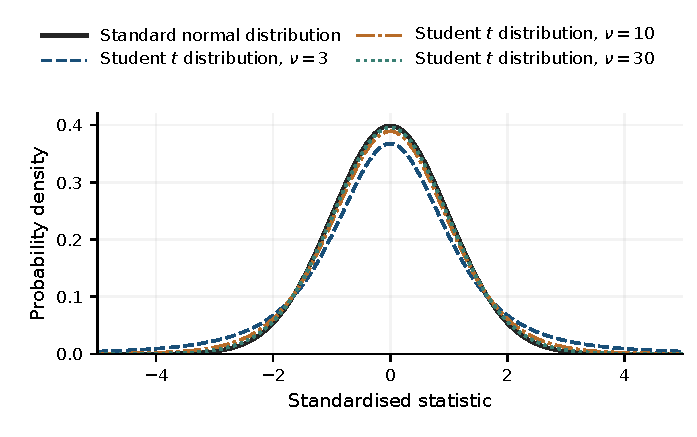
\includegraphics{focused_reference_distributions.pdf}
  \caption{Standard normal distribution and Student \(t\) distributions with 3, 10, and 30 degrees of freedom.}
  \label{fig:normal-student-t}
\end{figure}

Figure~\ref{fig:normal-student-t} shows that the Student \(t\) distribution
has heavier tails than the standard normal distribution, especially when
\(\nu\) is small, so a larger absolute statistic is needed to reject the
null at the same significance level.
As \(\nu\) increases, the Student \(t\) distribution approaches the
standard normal distribution, and their rejection cutoffs become closer.

For MI, the estimated variance contributions are \(\Vhat(P)/n_P\) and
\(\Vhat(Q)/n_Q\). The ordinary \(n_P-1\) and \(n_Q-1\) values follow
from the scaled chi-squared distribution of a sample variance when each
population has a normal distribution; they do not automatically apply to an
estimated pointwise-MI variance.
Chapter~\ref{chap:expanded} therefore derives the component degrees of
freedom from the sampling variability of \(\Vhat(P)\) and \(\Vhat(Q)\),
using the same moment-matching principle.

The estimated MI sampling variance \(\Vhat(P)/n_P\) describes uncertainty
in \(\Ihat(P)\), whereas \(\Var\{\Vhat(P)\}\) measures how much the
variance estimate itself changes between samples. Even variance estimators
with the same mean can have different sampling variances, so Satterthwaite's
calculation matches both moments. Greater sampling variance relative to the
squared mean gives fewer degrees of freedom and a larger rejection cutoff
\citep{satterthwaite1946}. A sample-size assignment alone does not adapt
to differences in this relative variability between probability tables.

The same principle has been used in regression to account for
uncertainty in estimated variances
\citep{panwall2002,bell2002,kauermann2001,fay2001,imbens2016}.
\citet{panwall2002} use Student \(t\) distributions and \(F\) distributions with
approximate degrees of freedom that account for the sampling variability
of a regression variance estimate to reduce excessive Wald rejection.
\citet{bell2002} examine both
bias reduction in the variance estimator and Satterthwaite degrees of
freedom, finding that each contributes to improved inference. Their
experiments also show that using Satterthwaite degrees of freedom with a
positively biased variance estimator can produce very conservative tests.
The distinction matters for MI: a larger cutoff can compensate for some
excessive rejection, but it does not change the estimated variance or
remove bias in the estimated MI difference.

\medskip
\thesisminiheading{Resampling alternatives.}

A bootstrap approximates sampling variation by repeatedly drawing samples
with replacement from the observed data \citep{efron1979}. For this
comparison, samples would be drawn separately from the two observed tables,
using their original sample sizes, and the MI difference recalculated for
each pair. Resampling from separate empirical probability tables allows
their cell probabilities to differ and provides an estimated sampling
distribution of the MI difference. The bootstrap
variation around the observed estimate could then be used to construct
an uncertainty interval for the population difference and assess whether
that interval includes zero.

Because an ordinary empirical bootstrap assigns an unobserved cell zero
probability, it cannot sample that cell and can therefore miss error
arising from unobserved cells. \citet{paninski2003} gives a broader warning: confidence
intervals based on resampling can be too narrow when information estimates
remain biased.

A simple permutation test combines the two samples and shuffles their
group labels, giving an exact test when the populations have the same
complete distribution, \(P=Q\). Our hypothesis requires only
\(I(P)=I(Q)\), allowing the tables to differ while their MI values are
equal. Equal MI alone therefore does not guarantee that this label-permutation test
has the stated false-positive rate \citep{chung2013}.
Although specialised permutation methods allow distinct populations in
some parameter comparisons \citep{janssen1997,chung2013}, their validity
for equal MI would need to be established.

\section{Previous work and this thesis's contribution}

Existing uncertainty calculations describe how much an MI estimate varies
between samples. \citet{roulston1999} derives entropy and MI error estimates
using error propagation and examines them numerically. The first-order
results of \citet{moddemeijer1989} and \citet{brillinger2004} give the MI
sampling variance as approximately \(V(P)/n_P\), as developed in
Section~\ref{sec:first-order-mi-background}.

In a segregation application, \citet{mora2009} derive an approximation using
a normal distribution for comparing positive population MI between
populations and time periods, providing a direct precedent for the Wald
test used as the baseline. Their later
peer-reviewed account places the MI index within the segregation literature
\citep{mora2011}.

Hutcheson's test provides a related precedent for comparing estimated
information quantities using a Student \(t\) distribution as an approximate
reference. It compares two estimates of Shannon diversity, or entropy,
using a Welch-type statistic with effective degrees of freedom
\begin{equation}
  \nu_H=
  \frac{(s_{H,P}^2+s_{H,Q}^2)^2}
       {(s_{H,P}^2)^2/n_P+(s_{H,Q}^2)^2/n_Q}
  \label{eq:hutcheson-df}
\end{equation}
\citep{hutcheson1970}. Here each of
\(s_{H,P}^2\) and \(s_{H,Q}^2\) is the estimated sampling variance of the
corresponding entropy estimator \(\widehat H\). The formula assigns the
two variance components degrees of freedom \(n_P\) and \(n_Q\), rather
than the \(n_P-1\) and \(n_Q-1\) values used in the ordinary Welch test.

For MI, the row, column, and joint entropies are calculated from the same
observations, so their estimation errors are connected through the cell
counts contributing to all three. The MI sampling-variance formulas in
Section~\ref{sec:first-order-mi-background} account for this dependence
when estimating uncertainty in MI.

In a Bayesian approach to uncertainty about population MI,
\citet{hutter2002} and \citet{hutterzaffalon2005} model the unknown cell
probabilities and calculate the variance and shape of the resulting MI
distribution conditional on the observed table. Our repeated-sampling
comparison instead asks how often the Wald test and the Expanded Welch
test reject equal MI when new samples are drawn from fixed populations
\(P\) and \(Q\).

MI has also been used to test whether complete population distributions
are equal. \citet{guha2014} compare two continuous distributions using MI
between pooled observations and their sample labels, while
\citet{drake2014} develop an MI-based \(k\)-sample test for discrete data.
This thesis compares the MI of two variables within each population,
testing \(I(P)=I(Q)\).

The additional calculation needed by the Expanded Welch test concerns how
much the estimated pointwise-MI variance changes between samples. The
moment-matching rule in Section~\ref{sec:welch-background} requires both
the sampling mean and variance of this estimate to obtain component
degrees of freedom.

This thesis derives a first-order approximation to that sampling variance
by tracking how changes in observed counts affect the estimated
pointwise-MI variance. A change in a cell count alters both the estimated
probability weights and the pointwise-MI values calculated from the joint
and marginal probabilities. Following the moment-matching approach used
in regression by \citet{panwall2002}, the Expanded Welch test uses this
sampling-variance approximation to obtain component degrees of freedom.
The component degrees of freedom are then combined using the
Welch--Satterthwaite rule.

The Wald test and the Expanded Welch test use the same estimated MI
difference and standard error, so their comparison isolates the effect of
changing the reference distribution.
The estimation problems identified by \citet{paninski2003} remain relevant:
residual bias can shift the estimated difference. For a fixed estimated
difference, an underestimated standard error can make the absolute test
statistic too large, while an overestimated standard error can make it
too small. The evaluation therefore
checks the variance-moment approximations separately from false-positive
rates and power.
